% Options for packages loaded elsewhere
\PassOptionsToPackage{unicode}{hyperref}
\PassOptionsToPackage{hyphens}{url}
\PassOptionsToPackage{dvipsnames,svgnames,x11names}{xcolor}
\PassOptionsToPackage{space}{xeCJK}
\documentclass[
  10pt,
]{article}
\usepackage{xcolor}
\usepackage[margin=0.72in]{geometry}
\usepackage{amsmath,amssymb}
\setcounter{secnumdepth}{-\maxdimen} % remove section numbering
\usepackage{iftex}
\ifPDFTeX
  \usepackage[T1]{fontenc}
  \usepackage[utf8]{inputenc}
  \usepackage{textcomp} % provide euro and other symbols
\else % if luatex or xetex
  \usepackage{unicode-math} % this also loads fontspec
  \defaultfontfeatures{Scale=MatchLowercase}
  \defaultfontfeatures[\rmfamily]{Ligatures=TeX,Scale=1}
\fi
\usepackage{lmodern}
\ifPDFTeX\else
  % xetex/luatex font selection
  \setmainfont[]{Cambria}
  \setmonofont[]{Consolas}
  \ifXeTeX
    \usepackage{xeCJK}
    \setCJKmainfont[]{Microsoft YaHei}
  \fi
  \ifLuaTeX
    \usepackage[]{luatexja-fontspec}
    \setmainjfont[]{Microsoft YaHei}
  \fi
\fi
% Use upquote if available, for straight quotes in verbatim environments
\IfFileExists{upquote.sty}{\usepackage{upquote}}{}
\IfFileExists{microtype.sty}{% use microtype if available
  \usepackage[]{microtype}
  \UseMicrotypeSet[protrusion]{basicmath} % disable protrusion for tt fonts
}{}
\makeatletter
\@ifundefined{KOMAClassName}{% if non-KOMA class
  \IfFileExists{parskip.sty}{%
    \usepackage{parskip}
  }{% else
    \setlength{\parindent}{0pt}
    \setlength{\parskip}{6pt plus 2pt minus 1pt}}
}{% if KOMA class
  \KOMAoptions{parskip=half}}
\makeatother
\usepackage{longtable,booktabs,array}
\newcounter{none} % for unnumbered tables
\usepackage{calc} % for calculating minipage widths
% Correct order of tables after \paragraph or \subparagraph
\usepackage{etoolbox}
\makeatletter
\patchcmd\longtable{\par}{\if@noskipsec\mbox{}\fi\par}{}{}
\makeatother
% Allow footnotes in longtable head/foot
\IfFileExists{footnotehyper.sty}{\usepackage{footnotehyper}}{\usepackage{footnote}}
\makesavenoteenv{longtable}
\usepackage{graphicx}
\makeatletter
\newsavebox\pandoc@box
\newcommand*\pandocbounded[1]{% scales image to fit in text height/width
  \sbox\pandoc@box{#1}%
  \Gscale@div\@tempa{\textheight}{\dimexpr\ht\pandoc@box+\dp\pandoc@box\relax}%
  \Gscale@div\@tempb{\linewidth}{\wd\pandoc@box}%
  \ifdim\@tempb\p@<\@tempa\p@\let\@tempa\@tempb\fi% select the smaller of both
  \ifdim\@tempa\p@<\p@\scalebox{\@tempa}{\usebox\pandoc@box}%
  \else\usebox{\pandoc@box}%
  \fi%
}
% Set default figure placement to htbp
\def\fps@figure{htbp}
\makeatother
\setlength{\emergencystretch}{3em} % prevent overfull lines
\providecommand{\tightlist}{%
  \setlength{\itemsep}{0pt}\setlength{\parskip}{0pt}}
\usepackage{bookmark}
\IfFileExists{xurl.sty}{\usepackage{xurl}}{} % add URL line breaks if available
\urlstyle{same}
\hypersetup{
  colorlinks=true,
  linkcolor={Maroon},
  filecolor={Maroon},
  citecolor={Blue},
  urlcolor={Blue},
  pdfcreator={LaTeX via pandoc}}

\author{}
\date{}

\renewcommand{\figurename}{图}
\begin{document}

\section{Eye Sentinel
同协议模型对照}\label{eye-sentinel-ux540cux534fux8baeux6a21ux578bux5bf9ux7167}

2026 年 11 月 18 日 · \href{backbone-comparison.en.md}{English} ·
\href{backbone-comparison.zh.pdf}{PDF}

\textbf{在 AIROGS 开发集上，同协议 ResNet-50 比 EfficientNet-B0 少漏诊
14 例。} 两种不确定性规则各复核 78 张原图，漏诊从 35 例降到 21
例，配对差值的 95\% 区间为 {[}-25, -3{]}，两者各留下 10
例误报。合并开发集的漏诊差为 -3 例，区间为 {[}-18, 12{]}。在 AIROGS
上加入质量分后，EfficientNet-B0 少漏 1 例，ResNet-50 多漏 2 例。

\subsection{训练对照}\label{ux8badux7ec3ux5bf9ux7167}

上一轮灰区分析中，历史 ResNet-50 在 AIROGS
上的漏诊较少。它使用原始训练数据，训练流程也与扩展版 EfficientNet-B0
不同。本轮在冻结的 \texttt{expanded\_20261113} 数据上补训
ResNet-50，沿用 EfficientNet-B0 的种子 20261117、65\%
原来源采样配额、50\%
混合退化概率、输入尺寸、批大小和优化器设置。两者各完成 2,400
次参数更新，比较各自第 2,400 步检查点。架构与相应的 ImageNet
初始化一并变化。

\subsection{开发集结果}\label{ux5f00ux53d1ux96c6ux7ed3ux679c}

AIROGS 有 773 张图，其中 380 张达到转诊标准。合并开发集有 2,053
张原图，其中 814
张按各来源标签定义为阳性。各模型使用对应验证集阴性分数的第 95
百分位作分类阈值，验证集规模分别为 767 和 2,046
张。每种规则在同一队列中复核相同数量，合并集为 206 张。

{\def\LTcaptype{none} % do not increment counter
\begin{longtable}[]{@{}
  >{\raggedright\arraybackslash}p{(\linewidth - 8\tabcolsep) * \real{0.29}}
  >{\raggedleft\arraybackslash}p{(\linewidth - 8\tabcolsep) * \real{0.1775}}
  >{\raggedleft\arraybackslash}p{(\linewidth - 8\tabcolsep) * \real{0.1775}}
  >{\raggedleft\arraybackslash}p{(\linewidth - 8\tabcolsep) * \real{0.1775}}
  >{\raggedleft\arraybackslash}p{(\linewidth - 8\tabcolsep) * \real{0.1775}}@{}}
\toprule\noalign{}
\begin{minipage}[b]{\linewidth}\raggedright
模型与复核规则
\end{minipage} & \begin{minipage}[b]{\linewidth}\raggedleft
AIROGS AUROC
\end{minipage} & \begin{minipage}[b]{\linewidth}\raggedleft
AIROGS 漏诊 / 误报
\end{minipage} & \begin{minipage}[b]{\linewidth}\raggedleft
合并 AUROC
\end{minipage} & \begin{minipage}[b]{\linewidth}\raggedleft
合并漏诊 / 误报
\end{minipage} \\
\midrule\noalign{}
\endhead
\bottomrule\noalign{}
\endlastfoot
EfficientNet-B0 · 不确定性 & 0.9744 & 35 / 10 & 0.9776 & 56 / 26 \\
EfficientNet-B0 · 加质量分 & 0.9744 & 34 / 11 & 0.9776 & 55 / 25 \\
同协议 ResNet-50 · 不确定性 & 0.9756 & 21 / 10 & 0.9766 & 53 / 26 \\
同协议 ResNet-50 · 加质量分 & 0.9756 & 23 / 10 & 0.9766 & 53 / 27 \\
历史 ResNet-50 · 不确定性 & 0.9818 & 14 / 9 & 0.9361 & 134 / 25 \\
\end{longtable}
}

AUROC
衡量整个开发队列的排序能力。漏诊与误报只统计复核名单之外的照片。疾病分数越接近分类阈值，按不确定性复核的优先级越高，距离在对数几率尺度上计算。质量规则再加
\texttt{1\ −\ q}，所以质量越低，复核优先级越高。\texttt{q} 由联合 EyeQ
与 FTHNet 模型给出，并截断到 0--1。

\newpage

\subsection{差值与训练过程}\label{ux5deeux503cux4e0eux8badux7ec3ux8fc7ux7a0b}

{\def\LTcaptype{none} % do not increment counter
\begin{longtable}[]{@{}
  >{\raggedright\arraybackslash}p{(\linewidth - 8\tabcolsep) * \real{0.29}}
  >{\raggedleft\arraybackslash}p{(\linewidth - 8\tabcolsep) * \real{0.1775}}
  >{\raggedleft\arraybackslash}p{(\linewidth - 8\tabcolsep) * \real{0.1775}}
  >{\raggedleft\arraybackslash}p{(\linewidth - 8\tabcolsep) * \real{0.1775}}
  >{\raggedleft\arraybackslash}p{(\linewidth - 8\tabcolsep) * \real{0.1775}}@{}}
\toprule\noalign{}
\begin{minipage}[b]{\linewidth}\raggedright
比较
\end{minipage} & \begin{minipage}[b]{\linewidth}\raggedleft
AIROGS 漏诊差
\end{minipage} & \begin{minipage}[b]{\linewidth}\raggedleft
AIROGS 总错误差
\end{minipage} & \begin{minipage}[b]{\linewidth}\raggedleft
合并漏诊差
\end{minipage} & \begin{minipage}[b]{\linewidth}\raggedleft
合并总错误差
\end{minipage} \\
\midrule\noalign{}
\endhead
\bottomrule\noalign{}
\endlastfoot
同协议 ResNet-50 减 EfficientNet-B0 & -14 {[}-25, -3{]} & -14 {[}-26,
-1{]} & -3 {[}-18, +12{]} & -3 {[}-21, +13{]} \\
EfficientNet-B0 加质量分 & -1 {[}-3, +3{]} & +0 {[}-3, +5{]} & -1 {[}-4,
+3{]} & -2 {[}-5, +5{]} \\
同协议 ResNet-50 加质量分 & +2 {[}+0, +6{]} & +2 {[}+0, +6{]} & +0
{[}-3, +4{]} & +1 {[}-3, +5{]} \\
\end{longtable}
}

负值表示左列方法留下的错误较少。括号为 2,000 次按关联组配对重采样所得的
95\% 区间。每次重采样都为各规则匹配约 10\%
的复核容量。区间衡量这批开发照片的变异。种子间变异仍需补训估计。

\begin{figure}
\centering
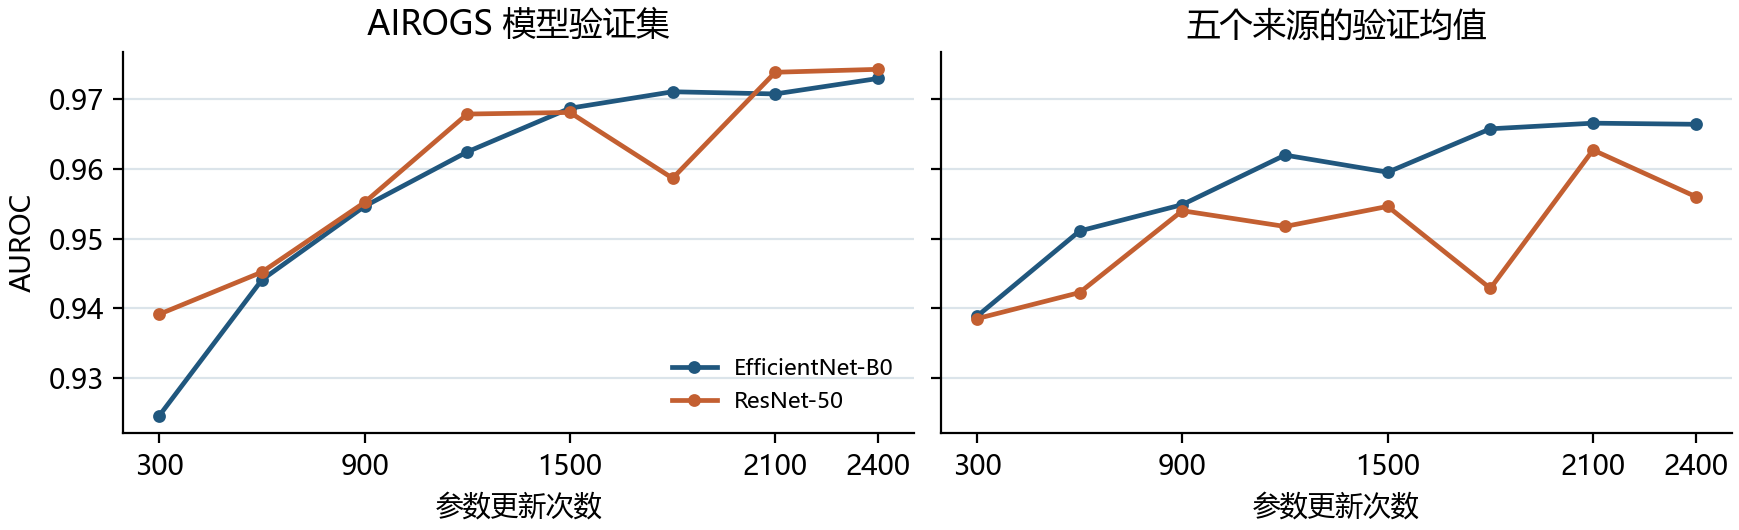
\includegraphics[width=0.96\linewidth,height=\textheight,keepaspectratio,alt={两种架构每 300 次更新的验证 AUROC。右图对既定的五个来源等权平均。}]{backbone-validation.zh.png}
\caption{两种架构每 300 次更新的验证
AUROC。右图对既定的五个来源等权平均。}
\end{figure}

两个模型的逐图采样次数、来源与类别分布、各类退化次数一致。每组训练共采样
38,384 次，其中 19,224 次施加合成退化。ResNet-50 用时约 21.5
分钟，混合精度训练跳过更新 0 次。第 2,400 步的 AIROGS 验证 AUROC 分别为
0.9729 和 0.9743。

\subsection{下一轮验证重点}\label{ux4e0bux4e00ux8f6eux9a8cux8bc1ux91cdux70b9}

先用另外两个既定种子复现 AIROGS
的漏诊差异，并检查合并队列是否也有收益。真实低质原图仍是独立缺口。上一轮开发集只有
12
张有人工低质标记的阳性原图，阴性为零。独立测试前仍需确定主队列、锁定阈值和复核规则，并明确阳性分流与同眼重拍后的处置。预留测试集继续封存。

\href{backbone-results.json}{汇总数据与输入哈希} ·
\href{../../../configs/backbone_20261118/resnet50.json}{训练配置} ·
\href{../../../tools/analyze_matched_backbones_20261118.py}{分析脚本} ·
\href{gray-zone.zh.md}{灰区评估}

\end{document}
